%%%%%%%%%%%%%%%%%%%%%%%%%%%%%%%%%%%%%%%%%%%%%%%%%%%%%%%%%%%%%%%%%%%%%%%%%%%%%%%%
%                                                                              %
%            A Painless Introduction to Programming UAMMD Modules              %
%                                                                              %
%%%%%%%%%%%%%%%%%%%%%%%%%%%%%%%%%%%%%%%%%%%%%%%%%%%%%%%%%%%%%%%%%%%%%%%%%%%%%%%%

\documentclass[a4paper,12pt,openany,hidelinks]{book}

\usepackage[hmarginratio=1:1]{geometry}
\usepackage{graphicx}
\usepackage{eso-pic}
\usepackage[utf8]{inputenc}
\usepackage{amsmath}
\usepackage{amssymb}
\usepackage{afterpage}
\usepackage{pagecolor}
\usepackage{picture}
\usepackage{comment}
\usepackage{listings}
\lstset{language = C++,
        frame = single,
        framextopmargin = 10pt,
        morecomment = [is]{\%!}{\^^M},
        basicstyle = \footnotesize,
        breaklines=true,
        postbreak=\mbox{$\hookrightarrow$\ }}
\usepackage{hyperref}
\hypersetup{
    colorlinks,
%    linkcolor={blue!50!black},
%    citecolor={red!50!black},
%    urlcolor={blue!80!black},
    pdftitle={A Painless Introduction to Programming UAMMD Modules},
    pdfauthor={M. Melendez},
    pdfsubject={UAMMD programming},
    pdfkeywords={molecular simulation, fluctuating hydrodynamics, UAMMD},
    pdfdisplaydoctitle
}

\begin{document}

%%%%%%%%%%%%%%%%%%%%%%%%%%%%%%%%%%%%  Head  %%%%%%%%%%%%%%%%%%%%%%%%%%%%%%%%%%%%

%%% Cover %%%

\thispagestyle{empty}
\newpagecolor{black}\afterpage{\restorepagecolor}

\AddToShipoutPicture*{
  \put(.5\paperwidth,.5\paperheight) {
    \makebox(0,0) {
      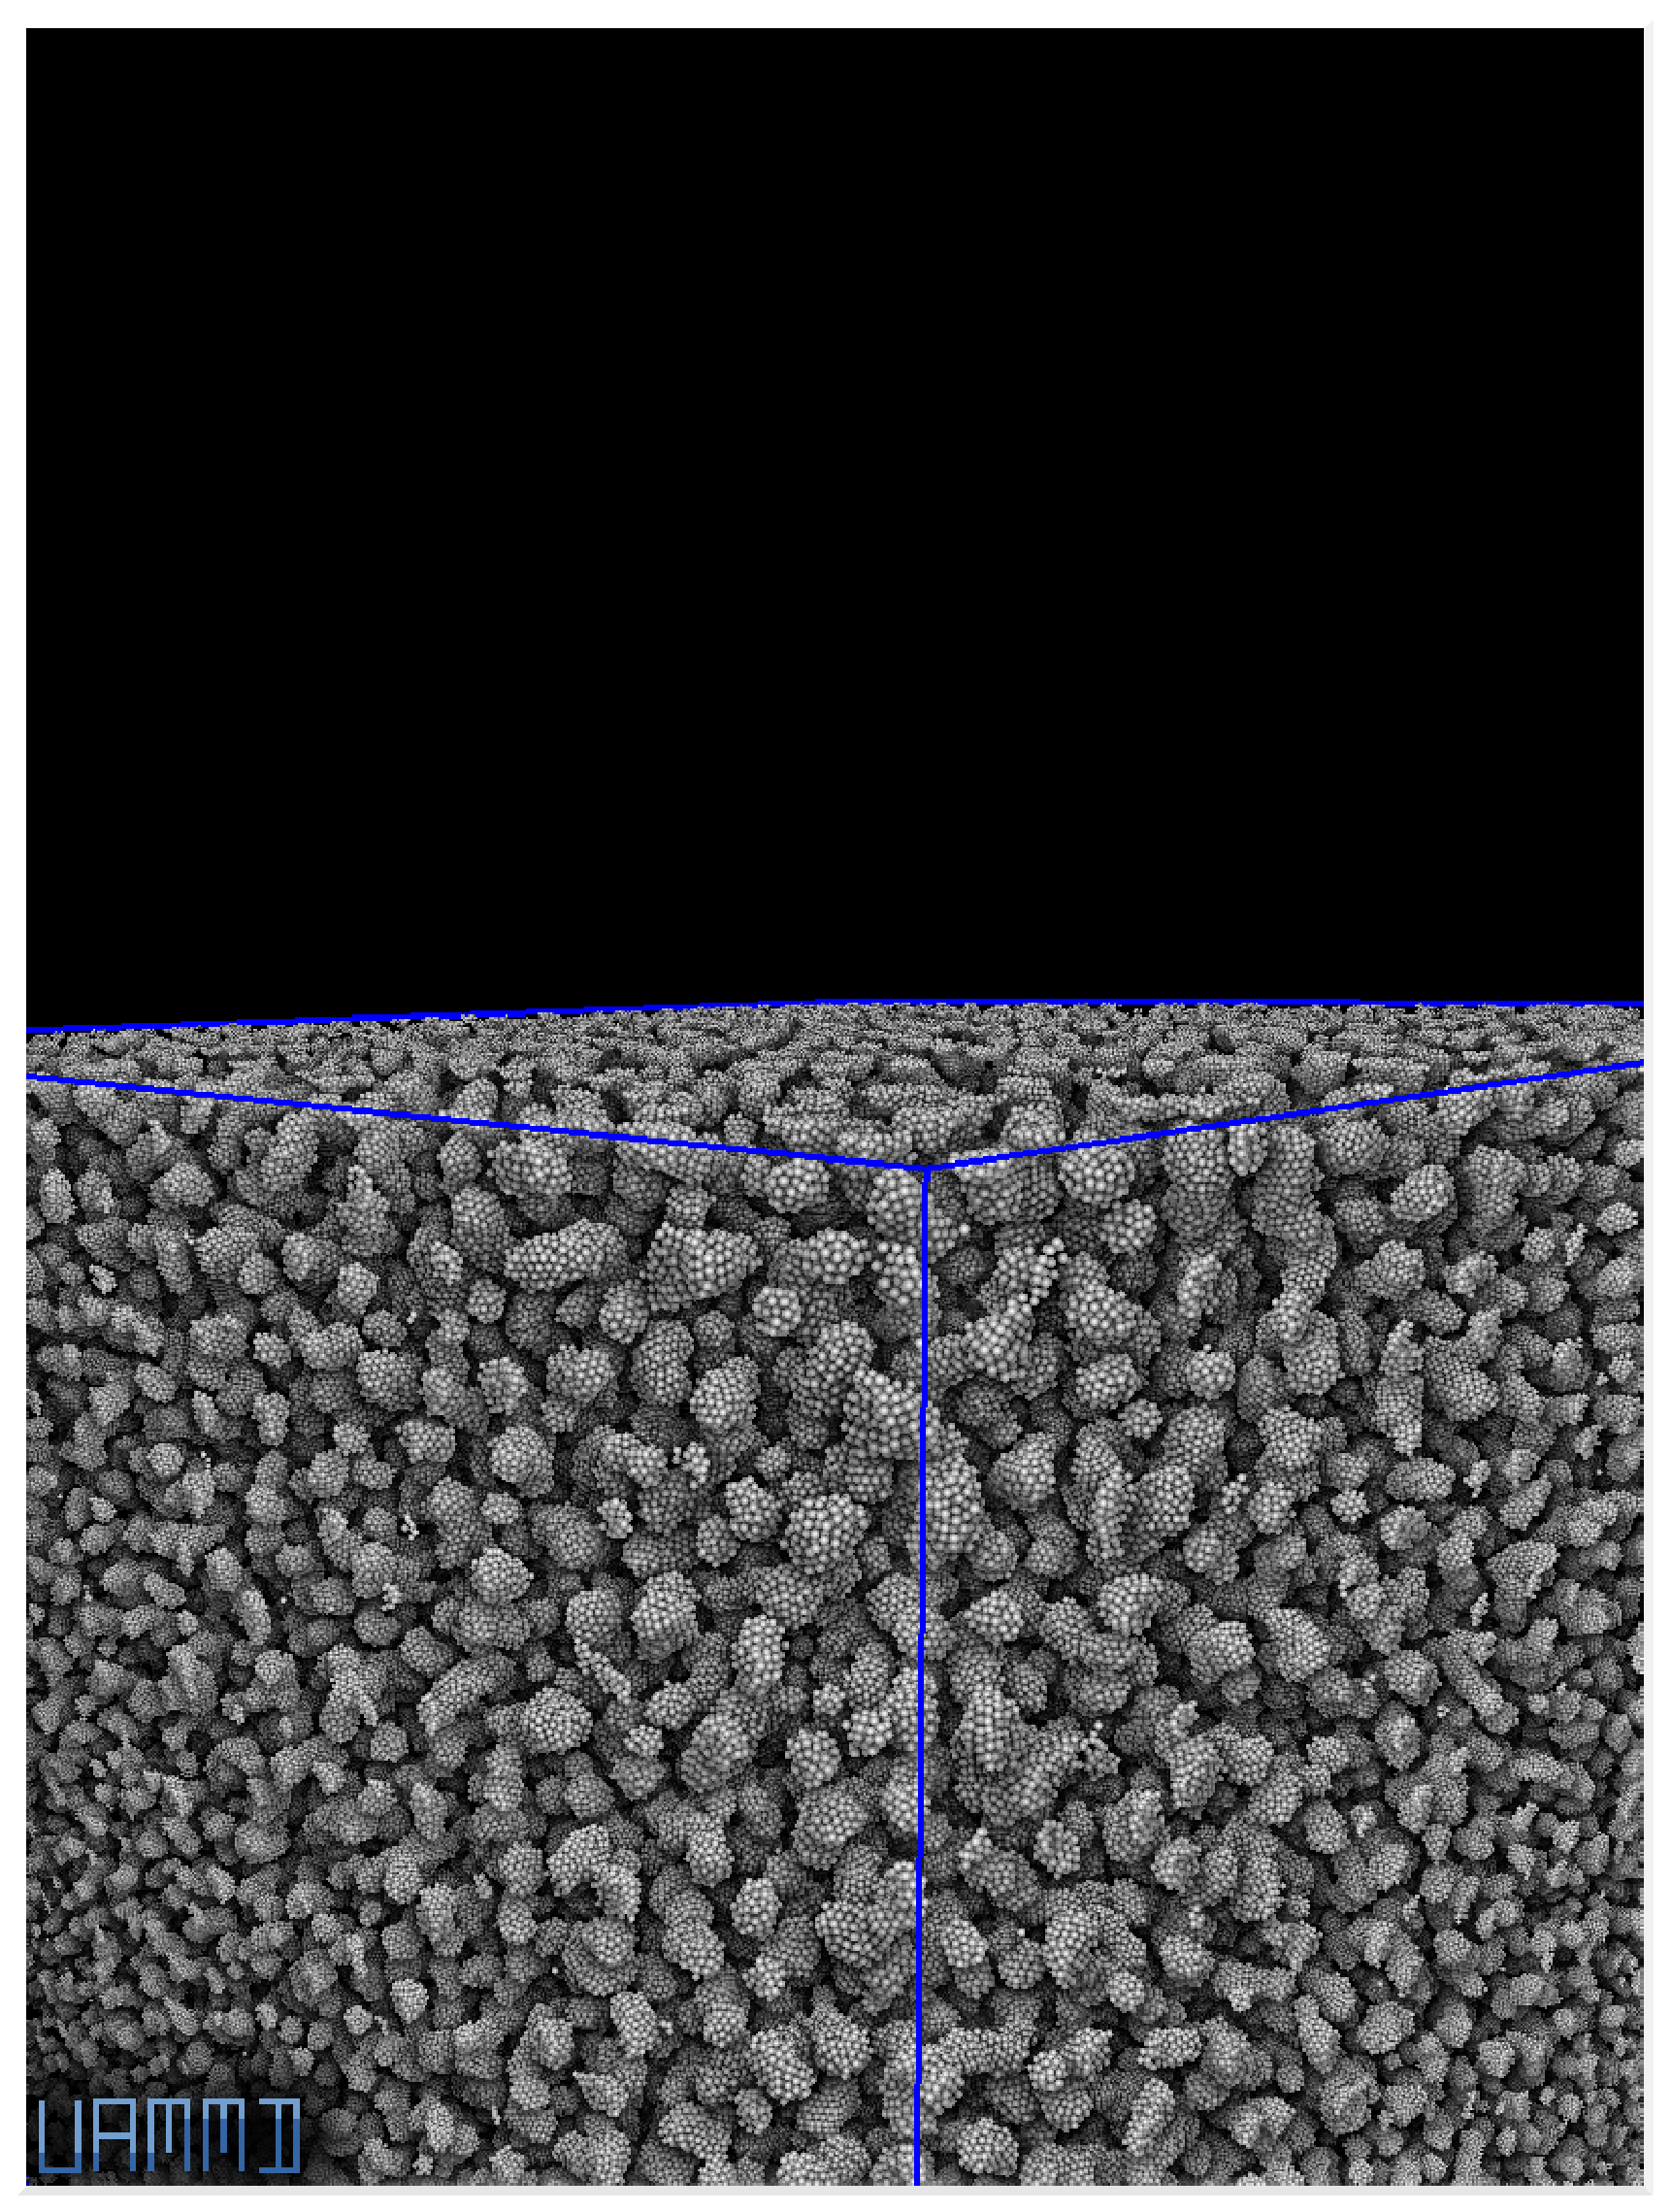
\includegraphics[width = 0.9 \paperwidth, keepaspectratio]{figures/uammd_intro_cover.eps}
    }
  }
}

\begin{center}
  {\color{white}
    \resizebox{0.8 \linewidth}{!}{\textbf{A Painless Introduction to}}

    \vspace{.5cm}

    \resizebox{\linewidth}{!}{\textbf{Programming UAMMD Modules}}
  }
\end{center}

\vspace{1.75cm}

\begin{center}
  {\huge {\color{white}Marc Mel\'endez Schofield}}
\end{center}

\vfill

\clearpage

\thispagestyle{empty}

\newgeometry{hmarginratio=2:3}


%%% Title page %%%

\title{A Painless Introduction to Programming UAMMD Modules}
\date{\today}
\author{Marc Mel\'endez Schofield}

\maketitle

%%%%%%%%%%%%%%%%%%%%%%%%%%%%%%  Copyright notice  %%%%%%%%%%%%%%%%%%%%%%%%%%%%%%


\thispagestyle{empty}


\noindent \textit{Title:} A Painless Introduction to Programming UAMMD Modules

\noindent \textit{Author:} Marc Mel\'endez Schofield. \\[1.2cm]

\vfill

\hrule

\vspace{2.0mm}

\noindent \includegraphics[height=0.75cm,clip=true]{figures/{by-nc-sa}.eps}
{\small Marc Mel\'endez Schofield (2020).} \\

{\small \noindent \textcopyright\ 2020,
Marc Mel\'endez Schofield. \textit{A Painless Introduction to Programming UAMMD
Modules} is distributed under the Creative Commons
Attribution-NonCommercial-ShareAlike 4.0 International
(\textsc{cc-by-nc-sa} 4.0). For summary and legal details visit: \\
\url{https://creativecommons.org/licenses/by-nc-sa/4.0/}}

%%%%%%%%%%%%%%%%%%%%%%%%%%%%%%%%%%%%  Body  %%%%%%%%%%%%%%%%%%%%%%%%%%%%%%%%%%%%

\tableofcontents

\chapter*{Introduction}
\markboth{INTRODUCTION}{INTRODUCTION}

\section*{On UAMMD}

The \textbf{Universally Adaptable Multiscale Molecular Dynamics} project,
known as \textbf{UAMMD}, collects molecular simulation algorithms for Graphics 
Processing Units (GPUs) into header-only code. In layman's terms, this means 
that you can write programs in CUDA and include high-performance algorithms to 
carry out rigorous classical dynamics many-body simulations. UAMMD relies on the 
GPU's capacity to perform huge amounts of analogous computations in parallel to 
increase the speed at which it works out many-body interactions.

The program was written mostly by Ra\'ul P\'erez Pel\'aez as a PhD candidate at
UAM, in Madrid. As a consequence, it became strongly focused on the interests of
the author. If you would like to use UAMMD to carry out some particular type of
simulation like, say, ReaxFF molecular dynamics, then you will probably have to
code it yourself. However, he did implement some very advanced modules for
fluctuating hydrodynamics so, if your research lies on that path, you will
definitely want to check out UAMMD. In my view, the great strength of UAMMD
comes from the abstract methods it provides to deal with many-body interactions
on the GPU, allowing you to quickly write simple but extremely efficient
simulations.

As the title of this book states, I aim to provide you with a painless 
introduction to writing UAMMD modules. I am writing with our research group's 
students in mind, imagining that you have begun to learn about molecular
simulation and have some (but not much) background in physics and programming.
If you need a more advanced approach, refer to the Wiki pages on the UAMMD
repository. Even if you don't, but you feel a painfully slow progress reading
this book, please skim through the pages and skip ahead until you find an
interesting section.

\section*{Beginner C++}

This section would be a good example of a chunk of text that you can skip and 
still be fine, as long as you have some very basic knowledge of what a C or C++ 
program looks like. The point here is \textit{not} to teach you C++, but rather 
to give you some basic feel for the language allowing you to read on and 
understand the gist of the code boxes. That should be enough for experimenting 
by tweaking the examples given here. You will, of course, eventually have to 
learn some CUDA if you wish to write advanced UAMMD programs, but there is a 
whole sea of free online resources out there. Instead of sailing out, it might 
be a good idea to understand what you want to know first (if your desires draw 
you out to sea, by all means go forth and sail!).

Below, I have copied the iconic ``Hello, World'' program, written for C++. It
begins by including input/output functionality by adding the \texttt{iostream}
standard library to our program (\texttt{iostream} contains \texttt{cout} and
texttt{endl} used a few lines down). We then specify that we will be using
the standard (txttt{std}) versions of \texttt{cout} and \texttt{endl}, which
saves us from having to write \texttt{std::cout} or \texttt{std::endl} each
time we want to mention them.
\begin{lstlisting}
%! codefile: code/helloworld.cpp
# include <iostream>

using std::cout;
using std::endl;

%! codeinsert: functionDefinitions
int main(int argc, char * argv[])
{
  cout<<"Hello, World!"<<endl;
  %! codeinsert: multiplesOfThree
  %! codeinsert: functionCalls
	return 0;
}
%! codeend
\end{lstlisting}

The final lines of code implement the \texttt{main} function. C++ programs
always execute this function first.

To define a function, we write the return value first, then the function name
followed by a list of arguments in parentheses. The contents come after the
arguments, so functions look like this:
\begin{lstlisting}
returnvalue functionname(list, of, arguments)
{
  what the function does
}
%!
\end{lstlisting}

Our ``Hello, World'' \texttt{main} function returns an integer (\texttt{int})
value: zero, in fact. As you can see, the function ends with \texttt{return 0;}.
Note that instructions end with a semicolon (;). The main function arguments, an
integer called \texttt{argc} and an array of strings called \texttt{argv}, refer
to the number of command-line arguments and the arguments themselves with which
the program was executed. In the next chapter, we will be passing these values
on to a UAMMD function that will deal with them. Here, we just ignore them.

The remaining line directs the ``\texttt{Hello, World!}'' string to standard
output, so that it would typically be printed on the screen, followed by an
end of line.

Compile the code above with \texttt{g++ helloword.cpp -o helloworld}, or
something similar. Running the program should print ``Hello, World!'' on the
screen.

The compiler ignores anything you write between \texttt{/*} and \texttt{*/}, so
you can use these characters to insert explanatory comments in your code. In a
typicaly program, you will declare variables, data structures and classes, on
which you will later carry out some calculations. UAMMD code might include lines
like these.
\begin{lstlisting}
int numberOfParticles; /* An integer value */
real temperature; /* A floating-point real value */
Box simulationBox(10); /* A cubic box of side 10 units */
bool printPositions; /* A boolean (true or false) value */
%!
\end{lstlisting}

We will control program flow with \texttt{for} and \texttt{if}. A \texttt{for}
loop like
\begin{lstlisting}
  for(int i = 1; i <= 100; ++i) {
    cout<<"Iteration: "<<i<<endl;
  }
%!
\end{lstlisting}
will begin by setting the integer \texttt{i} equal to 1. It will then execute
the \texttt{cout} code on the line below time and again while \texttt{i} does
not exceed \texttt{100}. After each iteration of the code, it will increase the
variable \texttt{i} by one (this is what \texttt{++i} does). Each time, it
prints out ``\texttt{Iteration:}'', followed by the value of \texttt{i}.

When you want the program to do something different depending on whether 
something else happened, you typically write code with the following structure.
\begin{lstlisting}
  if(this_is_true) {
    then_do_this();
    and_this();
  }
%!
\end{lstlisting}
Sometimes you want to specify what the program should do otherwise by adding
\begin{lstlisting}
  else {
    do_this_instead();
  }
%!
\end{lstlisting}
For example, suppose we wanted to print the number only every thirteen steps,
then we would replace the content of the for loop like this.
\begin{lstlisting}
%! codeblock: multiplesOfThree
  int printEverynSteps = 13;

  for(int i = 1; i <= 100; ++i) {
    if(printEverynSteps > 0
       && i % printEverynSteps == 0) {
        cout<<"Iteration: "<<i<<endl;
    }
  }
%! codeblockend
\end{lstlisting}
The \texttt{if} block says that if \texttt{printEverynSteps} is a positive 
number (\texttt{> 0}) and (\texttt{\&\&}) the remainder of the step number
divided by \texttt{printEverynSteps} equals zero (\texttt{step \%
printEverynSteps == 0}), then the line is printed. Compiling and
running the program outputs:
\begin{lstlisting}
Hello, World!
Iteration: 13
Iteration: 26
Iteration: 39
Iteration: 52
Iteration: 65
Iteration: 78
Iteration: 91
%!
\end{lstlisting}

Much of UAMMD code will be calling functions or methods defined elsewhere.
Let us add the following two functions before \texttt{main}.
\begin{lstlisting}
%! codeblock: functionDefinitions
int add(int a, int b) {
  return a + b;
}

void goodbye() {
  cout<<"Goodbye!"<<endl;
  return;
}
%! codeblockend
\end{lstlisting}
The first function takes two integers and returs their sum. The second takes no
arguments and returns none, but prints out ``Goodbye!''. To call these functions
after the \texttt{for} loop in our code, we simpy give their names followed by
their arguments in parentheses.
\begin{lstlisting}
%! codeblock: functionCalls
  cout<<"3 + 5 = "<<add(3,5)<<endl;
  goodbye();
%! codeblockend
\end{lstlisting}

\section*{Basic particle simulation}

Barometric distribution?

\section*{Installing CUDA}

\section*{Running code on liquid?}


\chapter{Our first UAMMD simulation}

Let us take the first step of our journey towards high-performance computing on
GPUs with a low-performance simple program that does hardly no computing. We
will modify a typical ``Hello, World!'' program in C++ slightly by adding a few
more lines (marked below with the comment \texttt{/* UAMMD */}). Note that we
also included the \texttt{using std::make\_shared} line so that we can later
declare \texttt{System} as a shared pointer (if you do not know what this means,
it doesn't matter right now).
\begin{lstlisting}
%! codefile: code/minimal.cu
# include "uammd.cuh" /* UAMMD */

using namespace uammd; /* UAMMD */
using std::make_shared;
using std::endl;
using std::cout;

int main(int argc, char *argv[]){

  auto sys = make_shared<System>(argc,argv); /* UAMMD */

  cout<<endl<<"--> Hello, UAMMD! <--"<<endl<<endl;

  sys->finish(); /* UAMMD */

  return 0;
}
%! codeend
\end{lstlisting}
Compile the code with
\begin{verbatim}
nvcc -O3 -I../uammd/src -I../uammd/src/third_party -o minimal
minimal.cu
\end{verbatim}
making sure that you replace the paths to UAMMD src code with the right path on
your system. Running \texttt{./minimal} outputs some UAMMD information, with
your ``Hello, UAMMD!'' message in the middle. Take out all the lines marked
\texttt{/* UAMMD */} and you are left with a typical ``Hello, World!'' program
in C++ that only outputs your message.

It might be helpful to go through the program to explain what each UAMMD line 
does in very general terms. You \texttt{include} the \texttt{uammd.cuh} header 
file and use the \texttt{uammd} namespace to have access to the functionality 
defined in the UAMMD source code. Within the main function, we enclose all our 
UAMMD code between the creation of a \texttt{System} and its destruction. The
\texttt{System} represents the computing environment in UAMMD. It deals with
access to the GPU and random number generation on the CPU, for example. In the
example above, we created a \texttt{System} named \texttt{sys} with
\begin{verbatim}
auto sys = make_shared<System>(argc,argv);
\end{verbatim}
and destroyed it at the end of the program with \texttt{sys->finish();}.

The program compiles and runs, but it feels like an empty sandwich. By expanding
it slightly, though, we can run a simple simulation.

\section{\label{physical_system}The physical system}

The main sandwich filling in our virtual kitchen has to be the physical system
that we wish to simulate, represented as a collection of particles. Define them
with the following lines after declaring \texttt{sys}.
\begin{lstlisting}
%! codeblock: particleData
  int numberOfParticles = 100000;
  auto particles
    = make_shared<ParticleData>(numberOfParticles, sys);
%! codeblockend
\end{lstlisting}
From now on, we have access to all the properties of our particles. We might, 
for example, decide to distribute the particles randomly within an imaginary 
128-unit box. In the following snippet, a code block set apart by brackets
defines \texttt{position} as a local variable, meaning that it cannot be
accessed from  other parts of the code, in contrast to \texttt{L}. Let it
replace the ``Hello, UAMMD!'' line above.\label{initialConditions}
\begin{lstlisting}
%! codeblock: initialConditions
  real L = 128;
  %! codeinsert: simulationBox

  {
    auto position
      = particles->getPos(access::location::cpu,
                          access::mode::write);

    for(int i = 0; i < numberOfParticles; ++i)
      position[i]
        = make_real4(sys->rng().uniform3(-0.5, 0.5), 0)*L;
  }
%! codeblockend
\end{lstlisting}
In the \texttt{for} loop we go over the list of positions and assign to each of
them a random four-dimensional vector. The first three components are random
numbers chosen from a uniform distribution between $-0.5$ and $0.5$ the last one
is zero. Because we then multiply the vector by \texttt{L}, we finally get
coordinates in the $-\frac{L}{2}$ to $\frac{L}{2}$ range. \texttt{L} was defined
as a \texttt{real} value. Depending on the options at compilation, this means
either a floating point or a double precision number. The final number in the
four-vector represents the particle type (here set to zero).

Making the position variable local guarantees that we will not read it later on,
thinking that we have access to the positions, but without having received the
updated values.

Suppose that, instead of writing to the particle positions, we wished to read
the velocities. The code snippet would resemble the box above, but we would call
\texttt{getVel} instead of \texttt{getPos} and indicate that we wish to read the
values.
\begin{lstlisting}
    auto velocities
      = particles->getVel(access::location::cpu,
                          access::mode::write);
%!
\end{lstlisting}
Other particle properties work similarly: use \texttt{getMass},
\texttt{getRadius}, \texttt{getCharge}, \texttt{getForce} or \texttt{getEnergy}.

Each particle is born with a name or identification number, which you may think
of as a serial number, accessible with the \texttt{getId} method. The reason why
you should care about this name concerns UAMMD reshuffling all the particles
every once in a while for efficiency. If you wish to track the trajectory of the
particle pointed at by \texttt{positions[3]}, you must remember that later on in
the code, when you get the positions with \texttt{getPos}, \texttt{positions[3]}
might be pointing at the location of a different particle.

Generally speaking, you will want to traverse the particle data in the order
provided by these \texttt{getWhatever} functions when you want to perform an
operation on all the particles, but don't care about the order, like when you
calculate the force on each particle. If you wish to track trajectories, for
example, then you need to identify the particles by name. So, if you would
like to print out the positions in the same order every time, use this:
\label{particlePositions}
\begin{lstlisting}
      auto position
        = particles->getPos(access::location::cpu,
                            access::mode::read);
      const int * index = particles->getIdOrderedIndices(access::location::cpu);

      out<<endl;
      for(int id = 0; id < numberOfParticles; ++id)
        out<<position[index[id]]<<endl;
%!
\end{lstlisting}
After getting the positions, you get a list of the indices ordered by name. Say
that you are searching for a particle with \texttt{id = 3}. Then
\texttt{index[id]} would tell you where it lies in the particle list, and
\texttt{position[index[id]]} would give you its position in space (and its type
as the fourth component of the position vector).

\section{Integrators}

The next ingredients adding flavour to our sandwich are time and motion. To get
the particles to move, we have to integrate their equations of motion
numerically. Now, we keep the new feature as simple as possible by assuming that
the particles do not interact, and treat them as atoms in an ideal gas.

We need some more functionality, which we import into our project with
\begin{lstlisting}
# include "Integrator/VerletNVE.cuh"
%!
\end{lstlisting}
at the beginning of the file, after including the \texttt{uammd.cuh} header
file. Now we can use the popular Verlet scheme to integrate the equations of
motion, but we need to set the values of some parameters first. \texttt{dt} sets
the size of the integration time step.
\begin{lstlisting}
%! codeblock: VerletParams
  using Verlet = VerletNVE::VerletNVE;
  Verlet::Parameters VerletParams;
  VerletParams.dt = 0.01;
  VerletParams.initVelocities=true;
  VerletParams.energy = 1.0;
%! codeblockend
\end{lstlisting}
In addition, we use the algorithm to initialise the velocities to random values
in such a way that the energy per particle equals \texttt{1.0}. Having set the
parameters, we activate the integrator with the following line.
\begin{lstlisting}
%! codeblock: Verlet
  auto integrator
    = make_shared<Verlet>(particles, sys, VerletParams);
%! codeblockend
\end{lstlisting}

Leaving their initial random positions, we allow the atoms to drift away. The 
program, we decide, will write the positions to \texttt{free\_expansion.dat}.
\begin{lstlisting}
%! codeblock: outputFile
  std::string outputFile = "free_expansion.dat";
  std::ofstream out(outputFile);

  int numberOfSteps = 1000;
  int printEverynSteps = 100;
%! codeblockend
\end{lstlisting}
Although we will tell the computer to calculate one thousand time steps, we
will only record the state of the system once every one hundred steps. 

To advance the system in time, use the integrator's \texttt{forwardTime} method.
\begin{lstlisting}
%! codeblock: integration
  for(int step = 0; step < numberOfSteps; ++step) {
    integrator->forwardTime();

    if(printEverynSteps > 0
       && step % printEverynSteps == 1) {
      /* ... Output particle positions ... */
      %! codeinsert: printPositions
    }
  }
%! codeblockend
\end{lstlisting}
You can easily replace the comment above with the output code explained at the
end of section \ref{physical_system} (page \pageref{particlePositions}).

\begin{comment}
\begin{lstlisting}
%! codefile: code/free_expansion.cu
# include "uammd.cuh"
# include "Integrator/VerletNVE.cuh"

using namespace uammd;
using std::make_shared;
using std::endl;

int main(int argc, char *argv[]){

  auto sys = make_shared<System>(argc, argv);

  %! codeinsert: particleData

  %! codeinsert: initialConditions

  %! codeinsert: VerletParams

  %! codeinsert: Verlet

  %! codeinsert: outputFile

  %! codeinsert: integration

  sys->finish();

  return 0;
}
%! codeend
\end{lstlisting}
\end{comment}

We should now have a working, admittedly unexciting, simulation. It represents 
the free expansion of an ideal gas, initially confined to a box that for some 
reason disappeared magically at the start of the simulation. It makes for an 
unlikely candidate to represent a physical situation of real interest, but we 
can make it better. However, before we incorporate further improvements in our 
code, we must mention that UAMMD has other integration schemes implemented as 
well as Monte Carlo methods, and we will turn to some of them later on in this 
book. For readers already familiar with numerical simulation methods, here is a 
teaser list: Verlet-like NVT, Brownian dynamics (with and without hydrodynamic 
interactions), Force Coupling Method and Lattice Boltzmann.

\section{The simulation box}

Instead of simulating an ideal gas in a tiny room in which the walls have 
vanished suddenly, we might like to produce the bulk behaviour of an ideal gas. 
A customary and convenient molecular dynamics technique imposes periodic 
boundary conditions on the system. Suppose our little gas-filled box without 
walls represents only a small amount of gas lost in the midst of a huge 
container. How do we simulate the trillions upon trillions of gas particles that 
surround the small volume that we picked? Easy. We divide space up into 
imaginary boxes, one of which contains our system, and assume that all the other 
systems in other boxes behave similarly. In fact, we treat them all as 
identical.

In such a periodic system, the simulation box has no physical meaning apart from 
indicating the periodicity in different directions of space. Nothing special 
happens at the walls, and moving the box or the system as a whole has no effect 
on the physics. Particles may leave the simulation box and wonder into 
neighbouring boxes without feeling anything. Due to periodicity, of course, if a 
particle leaves through the left wall of the box, say, then an identical 
particle will simultaneously enter through the right wall.

You'll remember that we set up our system by spreading the particles out in a
cube of side \texttt{L}. Fill space with periodic images of this box with the
following code snippet after the ``\texttt{real L}'' declaration (see page
\pageref{initialConditions}).
\begin{lstlisting}
    Box box(make_real3(L, L, L));
    bool periodicityX = true, periodicityY = true,
         periodicityZ = true;
    box.setPeriodicity(periodicityX, periodicityY,
                       periodicityZ);
%!
\end{lstlisting}
The coordinates that your program should output really depend on your interests. 
Do you wish to follow the motion of the particles that started off in the 
simulation box, even if they have wondered off? Then print out the positions, as 
on page \pageref{particlePositions}. Do you, instead, prefer to concentrate on 
the contents of the simulation box? Then print out the positions of the images 
that lie within that box with
\begin{lstlisting}
  out<<box.apply_pbc(make_real3(position[index[id]]))<<endl;
%!
\end{lstlisting}
\begin{comment}
\begin{lstlisting}
%! codeblock: simulationBox
    Box box(make_real3(L, L, L));
    bool periodicityX = true, periodicityY = true,
         periodicityZ = false;
    box.setPeriodicity(periodicityX, periodicityY,
                       periodicityZ);
%! codeblockend
%! codeblock: printPositions
      auto position
        = particles->getPos(access::location::cpu,
                            access::mode::read);
      const int * index = particles->getIdOrderedIndices(access::location::cpu);

      out<<endl;
      for(int id = 0; id < numberOfParticles; ++id)
        out<<box.apply_pbc(make_real3(position[index[id]]))<<endl;
%! codeblockend
\end{lstlisting}
\end{comment}
For example, imagine an ideal gas trapped between two horizontal pistons which
are quickly yanked apart. The gas would expand freely in the vertical ($z$)
direction, but we could imagine a periodic system along the $xy$ plane. Hence,
we would represent this system by changing the value of \texttt{periodicityZ}
above to \texttt{false}. Fig. \ref{free_expansion} displays the final state of
the gas as produced by the simulation we have written above.

\begin{figure}
  \includegraphics[width = \textwidth]{figures/free_expansion.eps}
  \caption{\label{free_expansion}Free expansion of an ideal gas in the $z$
           direction. The system is periodic along the $xy$ plane. On the left,
           the black dots represent particles that were inside the simulation
           box at the start of the computation, and grey dots represent their
           periodic images. On the right, black dots point out the particles
           inside the simulation box at the end of the computation, while grey
           dots mark the positions of particles in other boxes.}
\end{figure}

\section{Interactions}

The final ingredient adding flavour to our beginner simulations concerns 
interactions among particles. Nothing very exciting happens while particles
cannot bounce off, repel or attract each other.

Concentrate on short-range forces.

Minimal image convention.

\begin{comment}
\begin{lstlisting}
%! codefile: code/Lennard-Jones.cu
# include "uammd.cuh"
# include "Integrator/VerletNVE.cuh"

using namespace uammd;
using std::make_shared;
using std::endl;

int main(int argc, char *argv[]){

  auto sys = make_shared<System>(argc, argv);

  %! codeinsert: particleData

  %! codeinsert: initialConditions

  %! codeinsert: VerletParams

  %! codeinsert: Verlet

  %! codeinsert: outputFile

  %! codeinsert: integration

  sys->finish();

  return 0;
}
%! codeend
\end{lstlisting}
\end{comment}

\section{Parameters}


\chapter{Unleash your potential}

\section{Harmonic bonds}

\section{Alternative types of bonds}

\section{External fields}

\section{Other potentials (DPD, SPH)}

\section{Defining your own potentials}


\chapter{Macroscopic quantities}

\chapter{The Langevin thermostat}

seeding the PRNG

Brownian Dynamics

Force-biased Monte Carlo


\chapter{Long-range interactions}

\chapter{Hydrodynamics}

\chapter{Advanced topics}

\end{document}

%! codefile: Makefile
all: tangle weave

tangle:
	txt2tangle uammd_intro.tex
	for file in `ls chapters/*.tex`; do txt2tangle $$file; done

weave:
	latex uammd_intro.tex
	dvips uammd_intro.dvi
	ps2pdf uammd_intro.ps
%! codeend

%! codefile: README.md
# A Painless Introduction to Programming UAMMD Modules

UAMMD stands for **Universally Adaptable Multiscale Molecular Dynamics**. You
can find the project at:

[https://github.com/RaulPPelaez/UAMMD]

%! codeinsert: OnUAMMD src: chapters/introduction.tex

%! codeend

%! codefile: code/README.md
# Example programs

## Introduction

  %! codeinsert: codelist src: chapters/introduction.tex

## Our first UAMMD simulation

  %! codeinsert: codelist src: chapters/first_simulation.tex

%! codeend
